\documentclass{standalone}
\usepackage{tikz}
\begin{document}
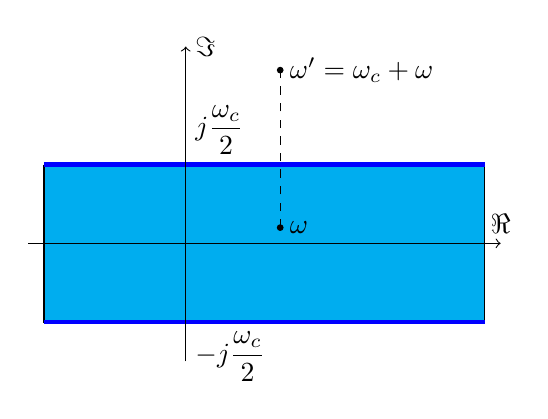
\begin{tikzpicture}[scale=2]
    \draw[fill=cyan](-0.9,0.5)--(1.9,0.5)--(1.9,-0.5)--(-0.9,-0.5)--(-0.9,0.5);
    \draw[-, blue,ultra thick](-0.9,0.5)--(1.9,0.5);       
    \draw[-, blue,ultra thick](-0.9,-0.5)--(1.9,-0.5);

    \draw[->](-1,0)--(2,0)node[above]{$\Re$};
    \draw[->](0,-0.75)--(0,1.25)node[right]{$\Im$};

    \node[above right]at(0,0.5){$\displaystyle j\frac{\omega_c}{2}$};
    \node[below right]at(0,-0.5){$\displaystyle -j\frac{\omega_c}{2}$};

    \filldraw[black](0.6,0.1)node[right]{$\omega$}circle(0.5pt);
    \filldraw[black](0.6,1.1)node[right]{$\omega'=\omega_c+\omega$}circle(0.5pt);
    \draw[dashed](0.6,0.1)--(0.6,1.1);
\end{tikzpicture}
\end{document}